\chapter{Introduction}
\fixme{Need to include measuring properties as motivation and intro, so that it leads to glass paper}

\fixme{Need to include more about GPUs in motivation}

\fixme{Finish writing motivation}

\label{sec:intro}
\section{Scope}

\begin{figure}
\centering
	 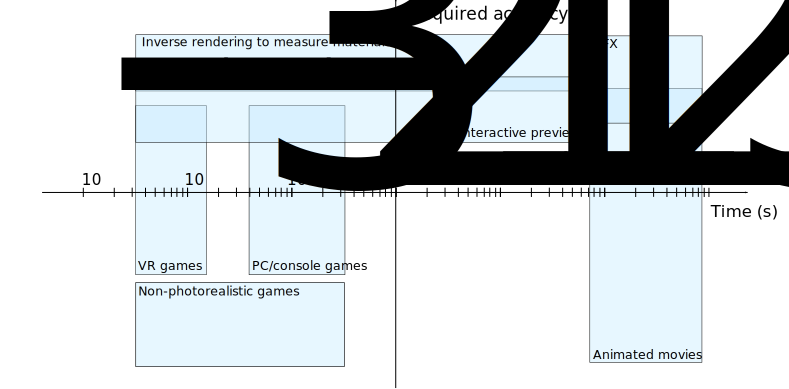
\includegraphics[draft,width=\textwidth]{figures/main_diagram}  \\
\caption{Some examples of photorealistic interactive rendering.} 
\label{fig:main_examples}
\end{figure}

The main goal of this thesis is to describe new techniques to bring movie production quality rendering into interactive applications.  The goal is to achieve photorealistic appearance as close as possible to the real world, while retaining the possibility for the user to interact with the simulation. In this thesis, we name these techniques "hybrid", as they combine techniques from the interactive world with accurate appearance models from physics and movie production pipelines.

Interactive realistic rendering applications are relevant in many fields, including
\begin{itemize}
\item 3D digital modeling and 3D printing,
\item Product development and visualization
\item Digital prototyping
\item Computer games and animation
\end{itemize}
In recent years, many advances have been made to achieve photorealistic quality in interactive applications,  but current techniques cannot achieve the photorealistic image quality that we see in movies. This thesis contributes with various techniques, exploring the area between interactive and real time rendering techniques (e.g. rasterization and interactive ray tracing), photorealistic rendering techniques (e.g. path tracing, hierarchical point cloud methods), and photorealistic appearance models (BRDFs and BSSRDFs, both analytical and measured). Our techniques, as most modern rendering techniques, are thought and developed to exploit the high throughput of graphic processing units (GPUs). Our contributions exploit both the long standing GPU hardware rasterization pipeline, but also focus on applications of the currently expanding field of interactive ray tracing. 

\section{Motivation}

\begin{figure}
\centering
	 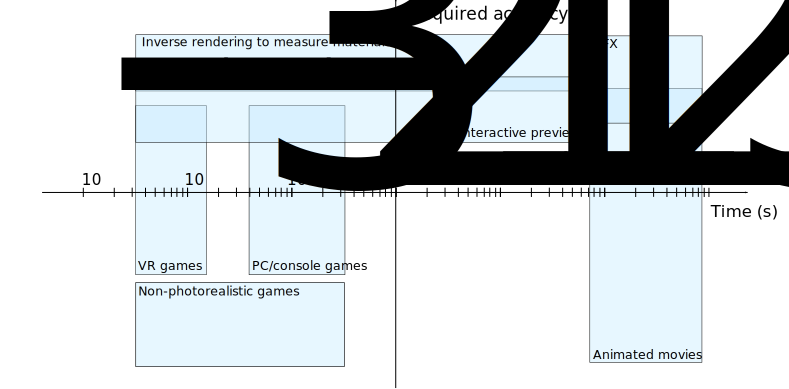
\includegraphics[width=\textwidth]{figures/main_diagram}  \\
\caption{Showing the continuum between interactive techniques, accurate techniques and photorealistic appearance.} 
\label{fig:main_diagram}
\end{figure}

Since the beginning of computer graphics, researchers have been striving to achieve more and more realistic renderings. Nowadays, for still images it is almost impossible to distinguish a rendering from an actual photograph. To achieve photorealistic images in various applications, usually a great amount of hours must be spent in modeling or acquiring the 3d geometry, choosing or matching the correct materials and actual rendering time to achieve the correct results. Especially in the rendering part, the more advanced the physical model used, the more time it takes to render. In the artistic process, many tweaks are often necessary to achieve a believable result. However, once this tweaks are made, a whole rendering cycle is needed to see the influence of the tweak on the final result. So, many applications display a preview of the final rendering result, and depending on the application the technique can be different. Some solutions are illustrated in Figure TODO. Compared to the final converged result TODO, we can simply display a noisy image that becomes less and less noisy with time TODO, post process the noisy image, or simplify the physical model TODO. All these techniques come with different trade offs, advantages and disadvantages. In general, these preview techniques introduce some sort of bias (i.e. the image is no longer physically correct) in exchange to getting rid of the noise. \

So, for these applications, where immediate feedback is important, there is a need in the industry to produce clever techniques that can exploit the existing constraints in order to deliver a more photorealistic result in the same rendering time. Of these constraints, the main is time, that can range to a few milliseconds per frame in a hard real time environment (games or virtual reality), to some fractions of a second (manifacturing) up to some minutes (artistic feedback, production, etc.). Other constraints may depend on the specific application: for example, the technique has to fit within a certain existing software architecture, or to specific hardware. As we mentioned in the previous section, we set to limit our scope to technique applicable to exploit the power of GPUs. These constraints may include the degree of photorealism necessary for the application. In some applications, the required photorealism can be limited: for example, in a video game, it is more important to get the perceptual "feel" of physically correct rather than a phyisically accurate result. In some other applications, the requirements are stricter: think architectural light simulation, where the architect need to know precisely how the light reacts to the different surfaces to see the overall illumination of the environment. We can visualize these constraints in a diagram, illustrated in figure TODO. On one axis, we have the photorealism of one technique. On the other axis, we have how fast the rendering time is for that specific technique. Each application can be thought as an area on this graph, so that a set of techniques (points on the graph) can fit the specific application.

In addition to the above motivations, we discuss three more detailed use cases in which there is a demand for improvements in photorealistic rendering techniques. These cases are not meant to be comprehensive of all applications in which interactive photorealistic rendering techniques are needed. However, they provide insights on possible industrial applications of the contributions in this thesis.

\begin{figure}
\centering
	 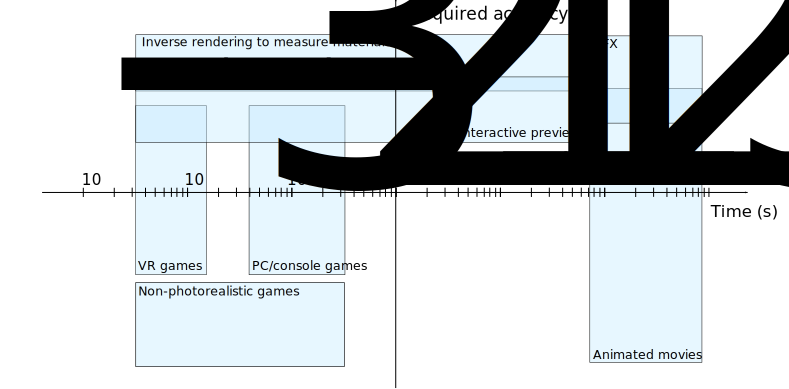
\includegraphics[draft,width=\textwidth]{figures/main_diagram}  \\
\caption{Applications of photorealistic interactive rendering. Left to right: 3d printing preview, architectural visualization, game prototyping.} 
\label{fig:applications}
\end{figure}

\subsection{3D printing}
The first case we discuss is additive manifacturing, in specific 3D printing. In this application, we would like to visualize the appearance of the printed object. Many challenges are required to faithfully represent a 3d printed object, depending on the process used: the most common techniques are extrusion and curing. In both this applications, the process greatly influences the shape and the appearance of the final object. In order to represent faithfully the appearance of the object, the printing material needs to be first faithfully measured or inferred. In general the materials used for 3d printing exhibit some particular radiometric properties, that makes them even more challenging to render accurately. 

In this application, the role of photorealistic rendering is dual. First, we can use photorealistic rendering to preview the final result of the 3d printing process. Secondary, we can actively use rendering to measure the radiometric properties of the object. In a specific setup and controller environment, a picture of the object is taken. Then, once a guess of the physical model is made, lots of different renderings can be made to predict the final appearance of the object. If a comparison can be made, we can effectively predict the radiometric properties of the final object. In both these applications, we require a high degree of photorealism, as we can see from the graph in Figure TODO. In this case, a noisier or downsampled result can be acceptable, both to give an idea of the final appearance or to measure the parameters. 

All these innovations go towards a more strict integration of 3D printing processes and digital image synthesis as a whole (The Digital-Physical Ecosystem). Photorealistic rendering helps reduce the number of iterations necessary to achieve a satisfying printed piece. This translates to reduced printing times for the same quality, and it avoids wasting potentially expensive printing material. Moreover, in a production environment, the validation though rendering allows to perform quality assurance on the finished pieces, by comparing them with previously printed versions of the same piece.

\subsection{Architectural visualization}

Our second case is architectural visualization. In this particular field, architects use interactive visualization tools to show how light propagates through a building, at different times of the day. This allows professionals to create buildings that best use natural illumination, minimizing the consumption due to electricity usage. In this particular application, an important focus is placed on an accurate representation of the materials, that can become increasingly complex. Materials used in construction are often radiometrically complex, with examples including frosted glass, marble or cloth. These materials can be either measured using some sort of apparatus, or matched by an artist so that they represent the appearance and light interaction properties of the original material. We place this application further TODO in our graph, since it requires a faster response time than the previous one, and a good physical accuracy as well. 

In this particular field, latest efforts have been put towards a more interactive experience, as to show the finished product to the project stakeholders. SO, a push in recent years has been done in architectural visualization for the customer, in particular in a virtual reality environment. Virtual reality pipelines need to maintain the same standard of physically based accuracy as the original simulation, while fitting into extreme time constraints, a handful of milliseconds per frame. Given the big performance challenge and the need of physical accuracy, fast techniques that exploit current hardware to achieve photorealistic visualization are needed.

\subsection{Computer games and animation}

A final application of fast interactive photorealisitic techniques is in computer games. Computer games have usually the strictest time constraints of all the applications so long presented. For a standard frame in a game, the industry standard is 16 milliseconds (60 frames per second). In recent year, virtual reality games are starting to become prominent, lowering the constraint to 7-11 milliseconds total (90-120 frames per second). Generically, games use triangle based rasterization, so that they can leverage custom hardware on GPUs. 

As games vary for gameplay, environment and style, photorealistic rendering can or cannot be employed in games. Still, a good number of games strives to achieve a realistic photorealistic look. However, in games the focus is on performance and the feel of realism, so the simulation is often inaccurate from a physical standpoint. Also, often the physical correctness is shelved in favor of more artistic control over the overall style. Given the hard time constraints, specific techniques need to be developed to achieve a realistic look. These techniques are often ad hoc solutions for a specific game, and no overall solution for all games exists. This makes it an interesting field to which contribute with general scalable physically based techniques, with the ultimate goal to reduce production costs.

\section{Outcome}

\begin{figure}
\centering
	 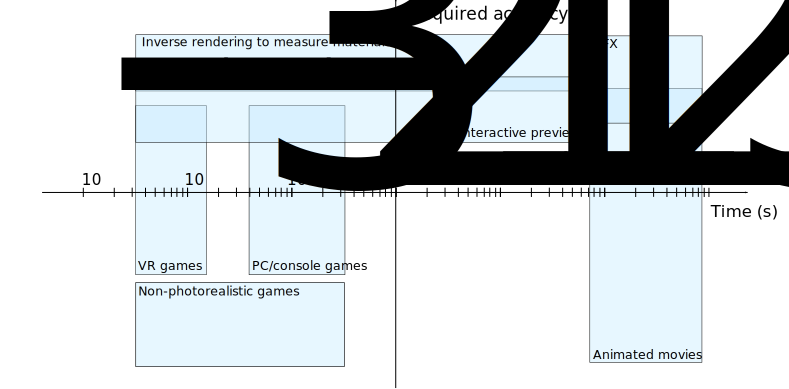
\includegraphics[draft,width=\textwidth]{figures/main_diagram}  \\
\caption{Main results from our papers.} 
\label{fig:main_results}
\end{figure}

During the three years period, we achieved a number of academic publications, reported at page~\pageref{sec:contributionlist}. In these publication, we managed to achieve a number of insights in the realm of computer graphics and material appearance. In particular, we created a range of techniques that can be readily applied to existing interactive applications. We believe we pushed the boundary on the degree of realism that can be achieved by modern GPUs on the same strict time constraints. 

In particular, papers~\ref{sec:interactivedirsss} and~\ref{sec:srt} achieve in this by providing widely applicable caching in the realm of interactive subsurface scattering and global illumination. Some examples of the results achieved in these papers are reported in Figure~\ref{fig:main_results}.

\section{Outline}

We report a list of all the contributions created during the course of the PhD studies at page~\pageref{sec:contributionlist}, including some unpublished notes, that we will refer mostly from Chapter~\ref{sec:background} to provide additional details. All the various publications are available as appendices. 

We divide our thesis into four main chapters. In Chapter~\ref{sec:background}, we first provide some background on some of the necessary foundations in radiometry, photorealistic appearance models and interactive rendering techniques. We will then provide in Chapter~\ref{sec:related} an overarching literature review on the current efforts of the rendering community to achieve photorealistic interactive rendering, referring to the individual contributions for more detailed related work. In Chapter~\ref{sec:contributions}, most importantly, we will go into more detail about the individual contributions and how each one of them contributes to reaching the outcome of the thesis. We will finally summarize our conclusions in Chapter~\ref{sec:conclusion}. 
